En la física de partículas, la supersimetría es una simetría hipotética propuesta que relacionaría las propiedades de los bosones y los fermiones. Aunque todavía no se ha verificado experimentalmente que la supersimetría sea una simetría de la naturaleza, es parte fundamental de muchos modelos teóricos, incluyendo la teoría de supercuerdas, la supersimetría también esconocida por \SUSY (\textbf{SU}per\textbf{SY}mmetry) siendo una de las teorías más populares que postulan la existencia de física más allá del \ME. 
\begin{figure}[h!]
\centering
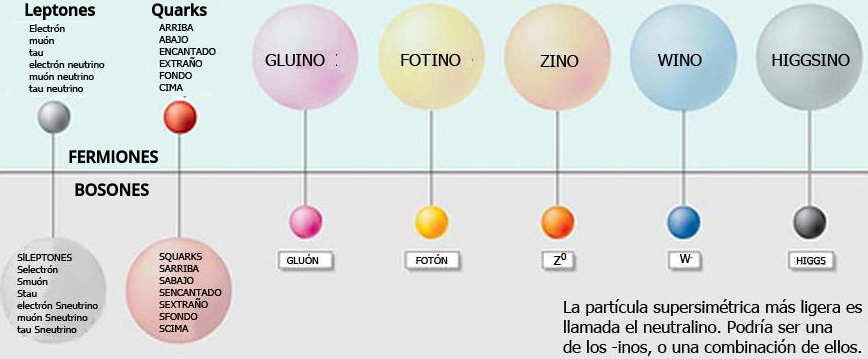
\includegraphics[width=.9\textwidth]{Analisis_y_Resultados/imagenes/supersimetrias.png}
\caption{Extensión del Modelo Estandar bajo la existencia de la supersimetría (\SUSY). %Página de origen : \href{http://www.cienciakanija.com/2009/11/13/confiamos-en-susy-lo-que-realmente-busca-el-lhc/}{\texttt{http://\-www.cienciakanija.com/\-2009/\-11/13/\-con\-fia\-mos-\-en-\-susy-\-lo-\-que-\-real\-men\-te-bus\-ca-el-lhc/}}.
}
\label{susy}
\end{figure}

De forma general el \ME ~se construye a partir de simetrías muy fundamentales que dan lugar a leyes de conservación, en el caso de \SUSY, esta incluye todas las simetrías que ya contiene el \ME~ y añade otra más que involucra al espín. Lo que postula \SUSY~ es que a cada partícula del \ME le corresponde un compañero supersimétrico que tiene el espín contrario, o sea, por cada fermión, \SUSY añade un bosón y por cada bosón añade un fermión. Por tanto, el número de partículas predicho por \SUSY es el doble que en el Modelo Estándar, como se visualiza en la Figura~\ref{susy}.

Se teoriza que \SUSY puede dar solución al problema de la materia oscura mediante su teorizada relación con la materia del \ME, en la mayoría de modelos de supersimetría, la partícula supersimétrica más ligera o \LSP (mencionada anteriormente) es necesariamente neutra y estable. Esto significa que nuestro Universo estaría lleno de estas partículas masivas, neutras y estables, que por tanto serían buenas candidatas a formar la materia oscura.

Sin embargo, debido a que dichas compañeras supersimétricas aún no han podido ser creadas en el laboratorio, sus masas deben ser mucho mayores que las de las partículas originales. Esto implica que la supersimetría, de ser cierta, está rota por algún mecanismo, la especificación de dicho mecanismo da lugar a diversas simplificaciones del \MSSM, donde algunas partículas supersimétricas, como el neutralino, podrían explicar el problema de la materia oscura del universo.

%Con la verificación de la existencia de \SUSY se consiguiria medir la masa de la \LSP seremos capaces de decir mucho más sobre si con SUSY es suficiente para explicar la materia oscura o si se necesita algo más.
La supersimetría (\SUSY) es una simetría espacio-temporal que mapea partículas y campos de espín entero (bosones) en partículas y campos de espín entero medio (fermiones), y viceversa. Los generadores $Q$ actúan como:
\begin{equation}
Q|\textsf{Fermion}> ~ = ~ |\textsf{Boson}> ~~ \textsf{y} ~~ Q|\textsf{Boson}> ~ = ~ |\textsf{Fermion}>
\end{equation}

Desde su propia definición, este operador tiene dos propiedades de gran alcance:
\begin{itemize}
\item[-] Cambia el spin de una partícula y como resultado sus propiedades espacio-temporales. Es por eso que la supersimetría no es una simetría interna sino una simetría de espacio-tiempo.
\item[-] En una teoría donde se realiza la supersimetría, cada estado de una partícula tiene al menos un supercompañero. Por lo tanto, en un entorno \SUSY, en lugar de estados de partículas individuales, uno tiene que lidiar con (super) múltiplos de estados de partículas.
\end{itemize}


